\talksection{Packetization Stage}

\begin{frame}{Packetization Overview}

\begin{itemize}
    \item Stage that does the actual vectorization: $<F, N> \rightarrow VF_N$
    \begin{itemize}
        \item Needs a vectorization factor $N$ (SIMD width)
        \item Calling $VF_N$ is like calling $F$, but $N$ times
        \item Straightforward thanks to preparation from previous stages
    \end{itemize}
    
    \item This is done per-instruction, for the whole function
    \begin{itemize}
        \item Instructions that define a value: define $N$ values, one for each instance
        \item Instructions with side effects: perform side effects for each instance
        \item New instruction has the same opcode but different types
    \end{itemize}
    
    \item Only \varying{varying} instructions need packetization
    \begin{itemize}
        \item \uniform{Uniform} instructions can remain scalar, executed once per work-group
        \item Requires \emph{Uniform Value Analysis} to know which instructions to vectorize
    \end{itemize}
    
\end{itemize}

\end{frame}

%%%%%%%%%%%%%%%%%%%%%%%%%%%%%%%%%%%%%%%%%%%%%%%%%%%%%%%%%%%%%%%%%%%%%%%%%%%%%%%%

\begin{frame}{Uniform Value Analysis}

\begin{itemize}
    \item Finds 'root' values
    \begin{itemize}
        \item \varying{Varying} values with no \varying{varying} operand
        \item Example: \varying{get\_global\_id(0)} has a different value for each isntance
    \end{itemize}
    \item Marks each IR value as \uniform{uniform} or \varying{varying}
    \begin{itemize}
        \item All values start as \uniform{uniform}
        \item Marking a value as \varying{varying} causes all users to also be marked \varying{varying}
        \item Marking is done recursively, starting with roots
        \item Values are marked before their users, to avoid cycles (phi nodes)
    \end{itemize}
\end{itemize}

\end{frame}

%%%%%%%%%%%%%%%%%%%%%%%%%%%%%%%%%%%%%%%%%%%%%%%%%%%%%%%%%%%%%%%%%%%%%%%%%%%%%%%%

\begin{frame}[fragile]{Uniform Value Analysis}

Example that combines \uniform{uniform} and \varying{varying} values:

\begin{codebox}[commandchars=\\\[\]]
kernel void add_uniform(global int *\uniform[dst], global int *\uniform[src], int \uniform[alpha]) {
    int \varying[tid] = \varying[get_global_id](0);
    \uniform[dst]\idx[\varying[tid]] = \uniform[src]\idx[\varying[tid]] + (\uniform[alpha] - \uniform[1]);
}
\end{codebox}

\begin{codebox}[commandchars=\\\[\]]
define void @add_uniform(i32* \uniform[%dst], i32* \uniform[%src], i32 \uniform[%alpha]) {
entry:
  \varying[%tid] = i32 \varying[@get_global_id(i32 0)]
  \varying[%arrayidx] = getelementptr i32* \uniform[%src], i32 \varying[%tid]
  \varying[%tmp] = load i32* \varying[%arrayidx], align 4
  \uniform[%sub] = sub i32 \uniform[%alpha], \uniform[1]
  \varying[%add] = add i32 \uniform[%sub], \varying[%tmp]
  \varying[%arrayidx2] = getelementptr i32* \uniform[%dst], i32 \varying[%tid]
  store i32 \varying[%add1], i32* \varying[%arrayidx2], align 4
  ret void
}
\end{codebox}

\end{frame}

%%%%%%%%%%%%%%%%%%%%%%%%%%%%%%%%%%%%%%%%%%%%%%%%%%%%%%%%%%%%%%%%%%%%%%%%%%%%%%%%

\begin{frame}[c]{UVA Example: Start}

\center{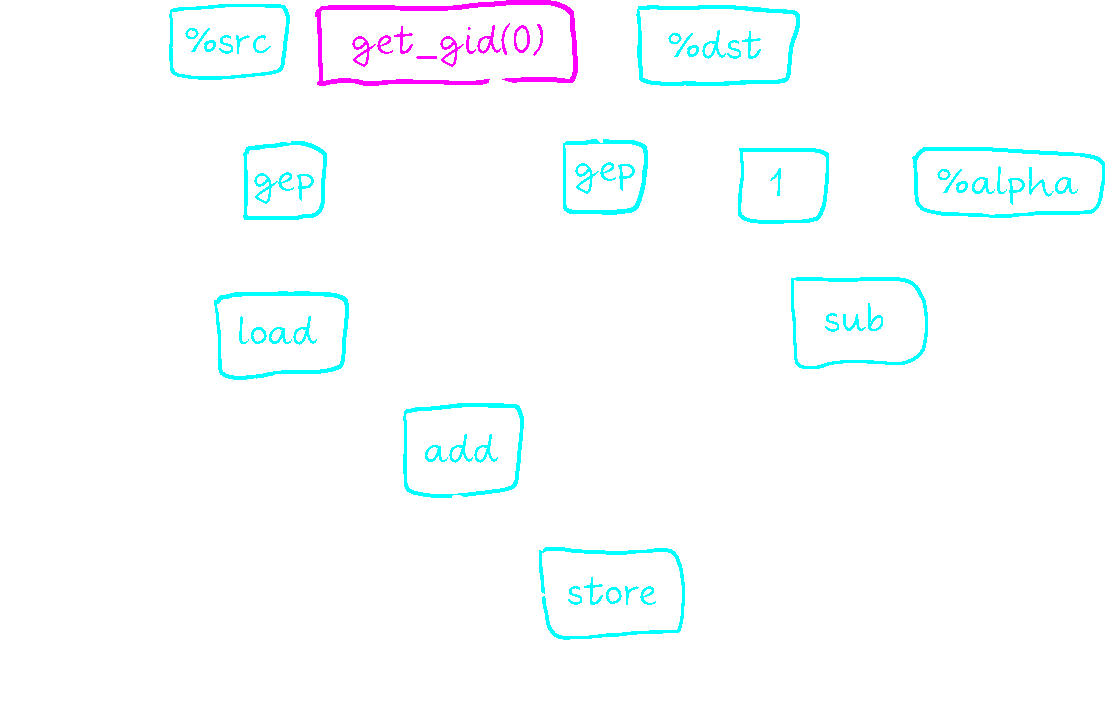
\includegraphics[scale=0.6]{images/uva-example-start.pdf}}

\end{frame}

%%%%%%%%%%%%%%%%%%%%%%%%%%%%%%%%%%%%%%%%%%%%%%%%%%%%%%%%%%%%%%%%%%%%%%%%%%%%%%%%

\begin{frame}[c]{UVA Example: Propagation}

\center{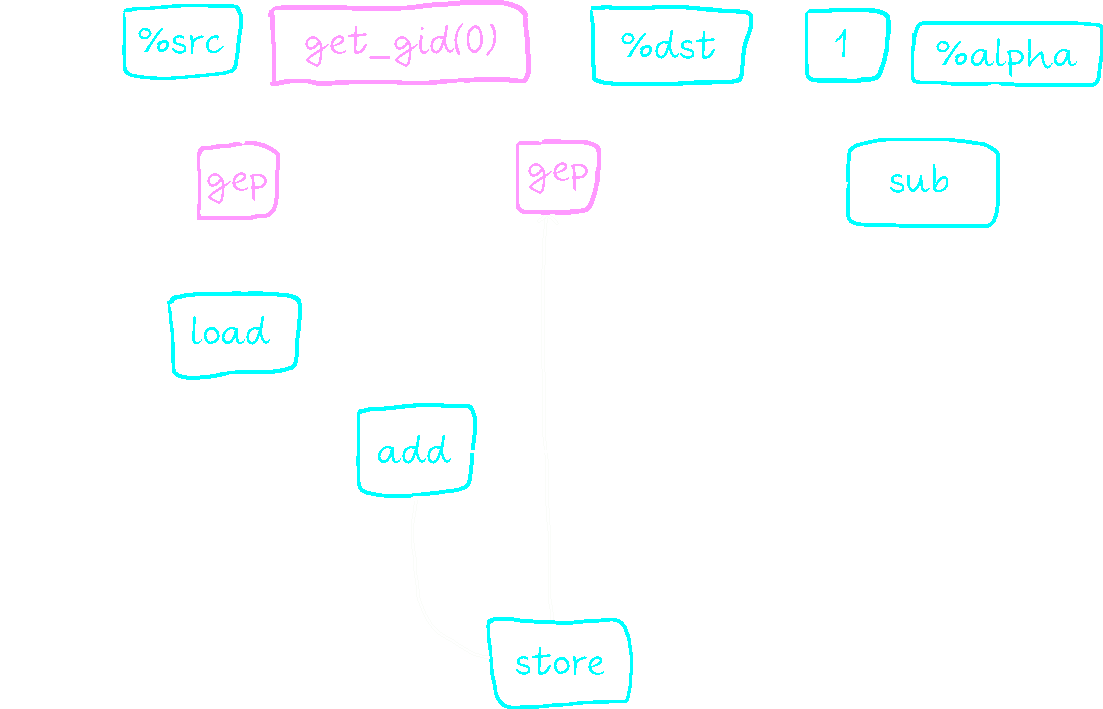
\includegraphics[scale=0.6]{images/uva-example-interm.pdf}}

\end{frame}

%%%%%%%%%%%%%%%%%%%%%%%%%%%%%%%%%%%%%%%%%%%%%%%%%%%%%%%%%%%%%%%%%%%%%%%%%%%%%%%%

\begin{frame}[c]{UVA Example: End}

\center{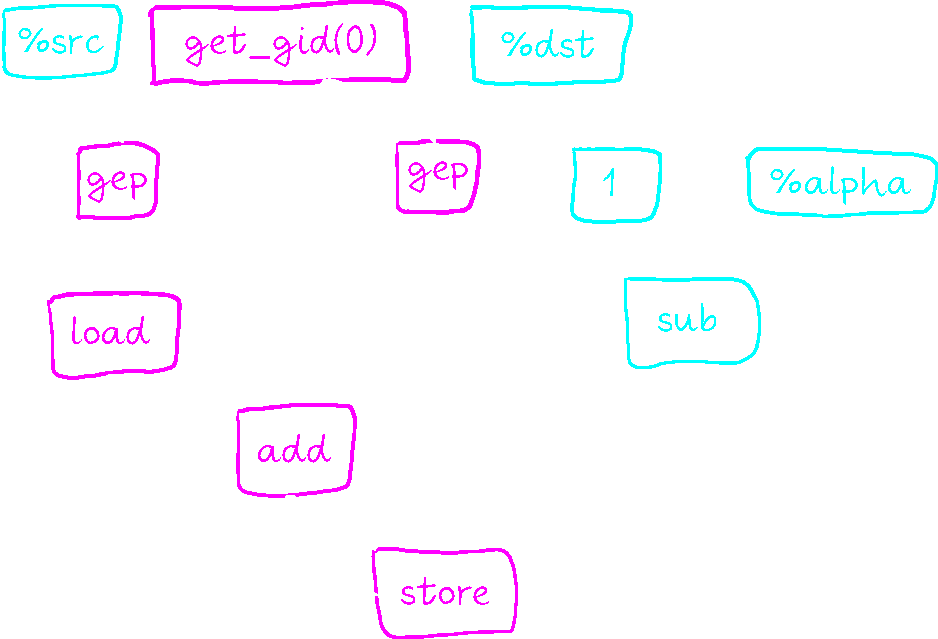
\includegraphics[scale=0.6]{images/uva-example-end.pdf}}

\end{frame}

%%%%%%%%%%%%%%%%%%%%%%%%%%%%%%%%%%%%%%%%%%%%%%%%%%%%%%%%%%%%%%%%%%%%%%%%%%%%%%%%

\begin{frame}{Memory Addressing}

\begin{itemize}
    %\item \varying{get\_global\_id(0)} was not packetized to a sequence of IDs. Why?
    \item Loads and stores are packetized according to the addressing mode
    \begin{itemize}
        \item Each operation can access $N$ memory elements
        \item Address usually has the form `\uniform{base} + \varying{offset}'
        \item Need to evaluate the offset for each of the $N$ lanes
    \end{itemize}
    
    \item How are these elements laid out in memory?
    \begin{itemize}
        \item The layout affects how operations are packetized
        \item Most common layouts can be described with a single \emph{stride}
    \end{itemize}
    
    \item Stride is the distance between successive elements
    \begin{itemize}
        \item Expressed in number of elements
        \item "How many elements are skipped in memory to get to the next one"
        \item One means elements are consecutive
        \item Negative means memory offsets are decreasing
    \end{itemize}
    
    %\item Not all kinds of memory operations can be expressed in IR
    %\begin{itemize}
    %    \item Generate calls to internal builtins
    %    \item Internal builtins can be implemented for each target as supported 
    %\end{itemize}
    
\end{itemize}

\end{frame}

%%%%%%%%%%%%%%%%%%%%%%%%%%%%%%%%%%%%%%%%%%%%%%%%%%%%%%%%%%%%%%%%%%%%%%%%%%%%%%%%

\begin{frame}[fragile]{Uniform Memory Addressing}

%% TODO: Use 1 as offset, update the diagram
\begin{itemize}
    \item Constant $Stride = 0$
    \item Packetized offset is \uniform{uniform} (e.g. $<0, 0, 0, 0>$)
    \item Transformed to a regular \emph{scalar} load or store
\end{itemize}

\begin{minipage}[t]{0.40\linewidth}
    \vspace{0.1ex}
    \begin{codebox}[commandchars=\\\[\]]

global int \uniform[*src];
int \uniform[x] = \uniform[src]\idx[\uniform[0]];






    \end{codebox}
\end{minipage}
\begin{minipage}[t]{0.49\linewidth}
    \begin{figure}
        
\includegraphics[scale=0.5]{images/uniform-access.pdf}
    \end{figure}
\end{minipage}

\end{frame}

%%%%%%%%%%%%%%%%%%%%%%%%%%%%%%%%%%%%%%%%%%%%%%%%%%%%%%%%%%%%%%%%%%%%%%%%%%%%%%%%

\begin{frame}[fragile]{Sequential Memory Addressing}

\begin{itemize}
    \item Constant $Stride = 1$
    \item Packetized offset is a sequence like $<0, 1, 2, 3>$
    \item Transformed to a regular \emph{vector} load or store
\end{itemize}

\begin{minipage}[t]{0.40\linewidth}
    \vspace{0.1ex}
    \begin{codebox}[commandchars=\\\[\]]

global int \uniform[*src];
int \varying[tid] = \varying[get_global_id(0)];
int \varying[x] = \uniform[src]\idx[\varying[tid]];





    \end{codebox}
\end{minipage}
\hspace{1em}
\begin{minipage}[t]{0.49\linewidth}
    \begin{figure}
        
\includegraphics[scale=0.5]{images/sequential-access.pdf}
    \end{figure}
\end{minipage}

\end{frame}

%%%%%%%%%%%%%%%%%%%%%%%%%%%%%%%%%%%%%%%%%%%%%%%%%%%%%%%%%%%%%%%%%%%%%%%%%%%%%%%%

\begin{frame}[fragile]{Interleaved Memory Addressing}

\begin{itemize}
    \item Constant $Stride > 1$
    \item Packetized offset is a sequence like $<0, 2, 4, 6>$
    \item Transformed to an \emph{interleaved} load or store
\end{itemize}

\begin{minipage}[t]{0.40\linewidth}
    \vspace{0.1ex}
    \begin{codebox}[commandchars=\\\[\]]
    
global int \uniform[*src];
int \varying[tid] = \varying[get_global_id(0)];
int \varying[even] = \uniform[src]\idx[\varying[tid] * \uniform[2]];
int \varying[odd] = \uniform[src]\idx[(\varying[tid] * \uniform[2]) + \uniform[1]];




    \end{codebox}
\end{minipage}
\hspace{1em}
\begin{minipage}[t]{0.49\linewidth}
    \begin{figure}
        
\includegraphics[scale=0.5]{images/interleaved-access.pdf}
    \end{figure}
\end{minipage}

\end{frame}

%%%%%%%%%%%%%%%%%%%%%%%%%%%%%%%%%%%%%%%%%%%%%%%%%%%%%%%%%%%%%%%%%%%%%%%%%%%%%%%%

\begin{frame}[fragile]{Arbitrary Memory Addressing}

\begin{itemize}
    \item Variable stride
    \item Packetized offset can be any sequence (e.g. $<0, 3, 7, 3>$)
    \item Transformed to a \emph{gather} load or \emph{scatter} store
\end{itemize}

\begin{minipage}[t]{0.40\linewidth}
    \vspace{0.1ex}
    \begin{codebox}[commandchars=\\\[\]]
    
global int \uniform[*src];
global int \uniform[*map];
int \varying[tid] = \varying[get_global_id(0)];
int \varying[x] = \uniform[src]\idx[\uniform[map]\idx[\varying[tid]]];




    \end{codebox}
\end{minipage}
\hspace{1em}
\begin{minipage}[t]{0.49\linewidth}
    \begin{figure}
        
\includegraphics[scale=0.5]{images/arbitrary-access.pdf}
    \end{figure}
\end{minipage}

\end{frame}

%%%%%%%%%%%%%%%%%%%%%%%%%%%%%%%%%%%%%%%%%%%%%%%%%%%%%%%%%%%%%%%%%%%%%%%%%%%%%%%%

\begin{frame}{Packetization Process}

\begin{itemize}
    \item Find leaves
    \begin{itemize}
        \item Leaves allow \varying{varying} values to 'escape' from the function, they are:
        \item Store instructions (\varying{varying} operand)
        \item Call instructions (\varying{varying} operand, or call has no use)
        \item Return instructions
    \end{itemize}
\end{itemize}

\begin{itemize}
    \item Recursively packetize leaves and their operands
    \begin{itemize}
        \item Broadcast \uniform{uniform} values (e.g. argument, constants)
        \item Replace \varying{get\_global\_id(0)} with a vector of IDs
        \item Packetize operands first, then instruction (top-down)
        \item Cache packetized values to prevent duplication
    \end{itemize}
\end{itemize}

\begin{itemize}
    \item Delete original scalar instructions if dead
\end{itemize}

\end{frame}

%%%%%%%%%%%%%%%%%%%%%%%%%%%%%%%%%%%%%%%%%%%%%%%%%%%%%%%%%%%%%%%%%%%%%%%%%%%%%%%%

\begin{frame}[c]{Packetization Example}

\center{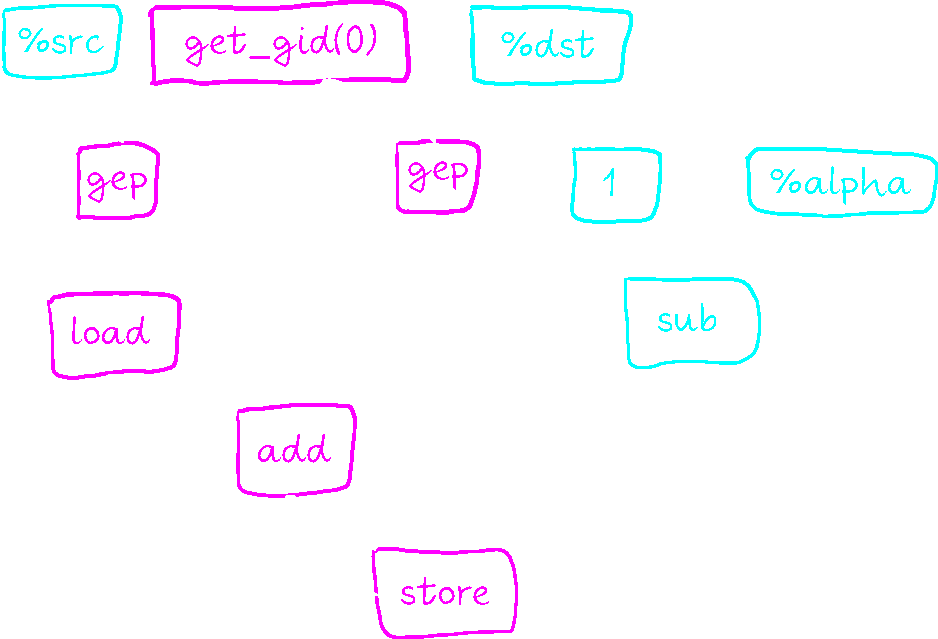
\includegraphics[scale=0.55]{images/uva-example-end.pdf}}

\end{frame}

%%%%%%%%%%%%%%%%%%%%%%%%%%%%%%%%%%%%%%%%%%%%%%%%%%%%%%%%%%%%%%%%%%%%%%%%%%%%%%%%

\begin{frame}[c]{Packetization Example}

\center{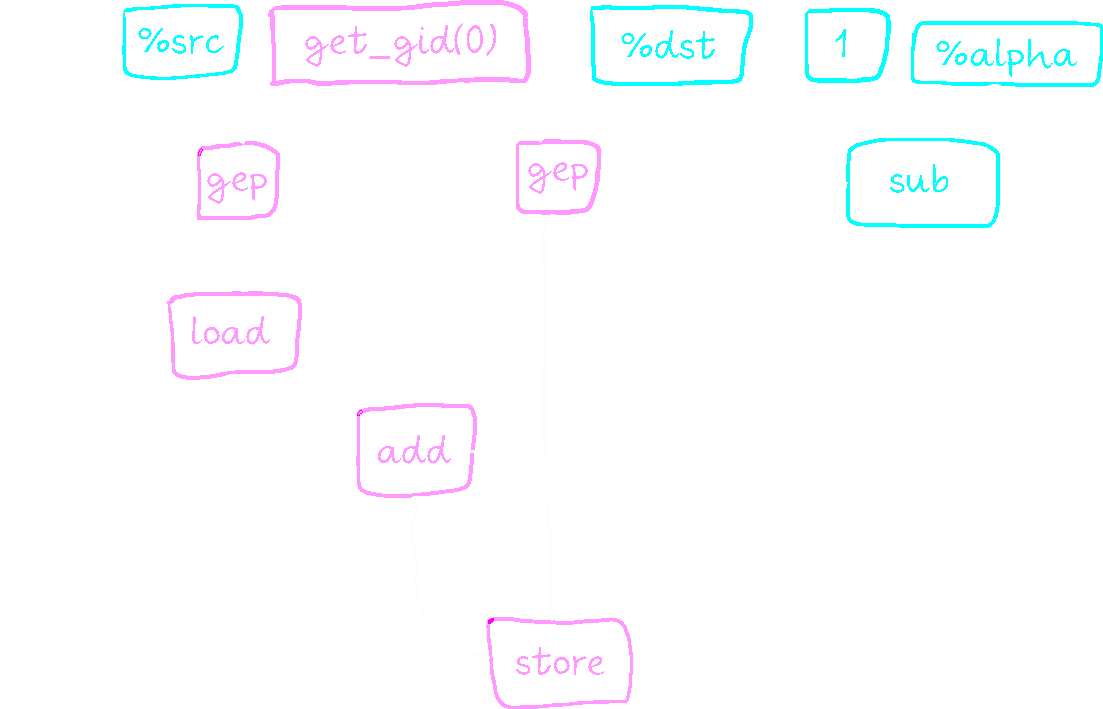
\includegraphics[scale=0.55]{images/packetization-1.pdf}}

\end{frame}

%%%%%%%%%%%%%%%%%%%%%%%%%%%%%%%%%%%%%%%%%%%%%%%%%%%%%%%%%%%%%%%%%%%%%%%%%%%%%%%%

\begin{frame}[c]{Packetization Example}

\center{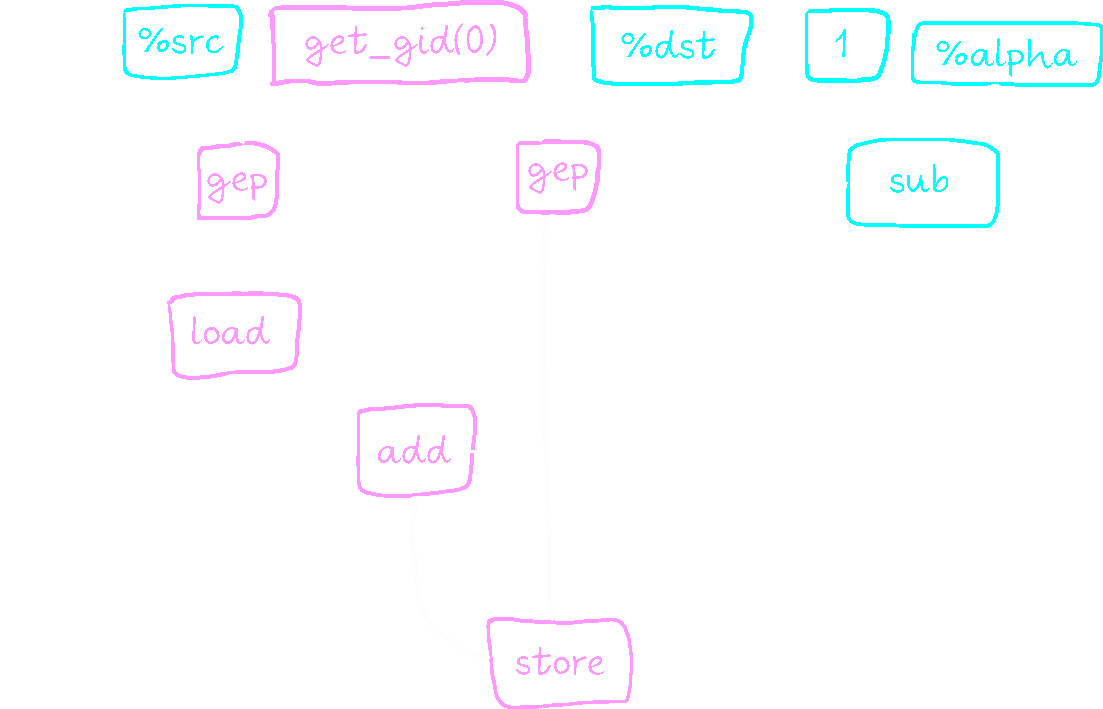
\includegraphics[scale=0.55]{images/packetization-2.pdf}}

\end{frame}

%%%%%%%%%%%%%%%%%%%%%%%%%%%%%%%%%%%%%%%%%%%%%%%%%%%%%%%%%%%%%%%%%%%%%%%%%%%%%%%%

\begin{frame}[c]{Packetization Example}

\center{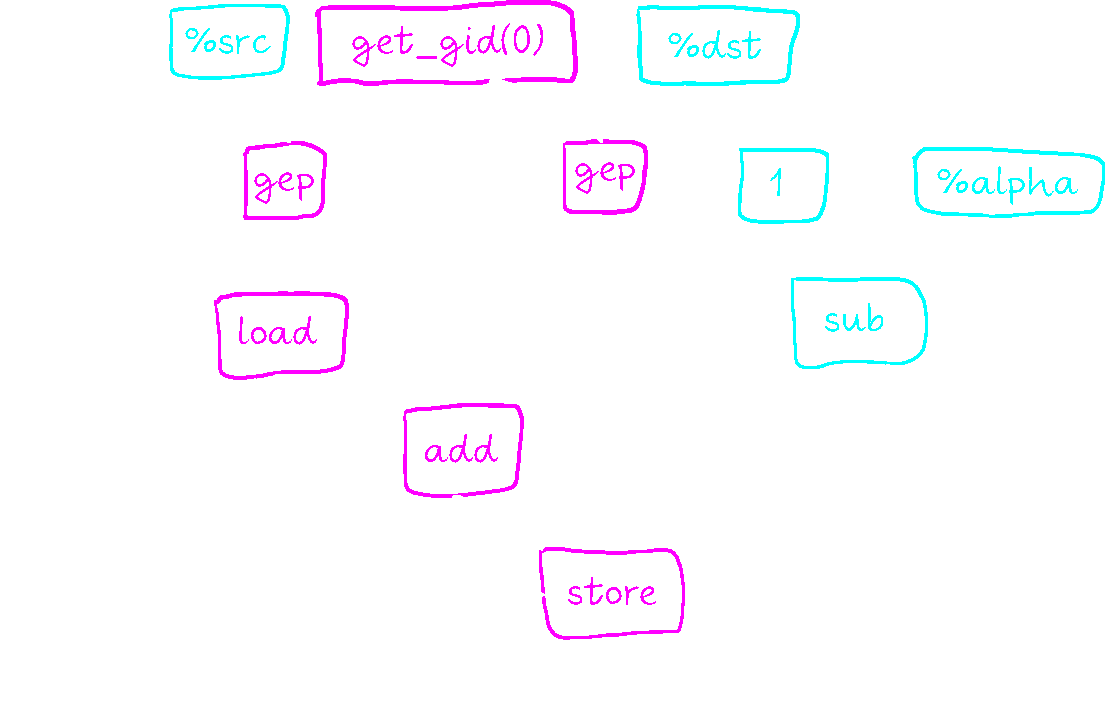
\includegraphics[scale=0.55]{images/packetization-3.pdf}}

\end{frame}

%%%%%%%%%%%%%%%%%%%%%%%%%%%%%%%%%%%%%%%%%%%%%%%%%%%%%%%%%%%%%%%%%%%%%%%%%%%%%%%%

\begin{frame}[c]{Packetization Example}

\center{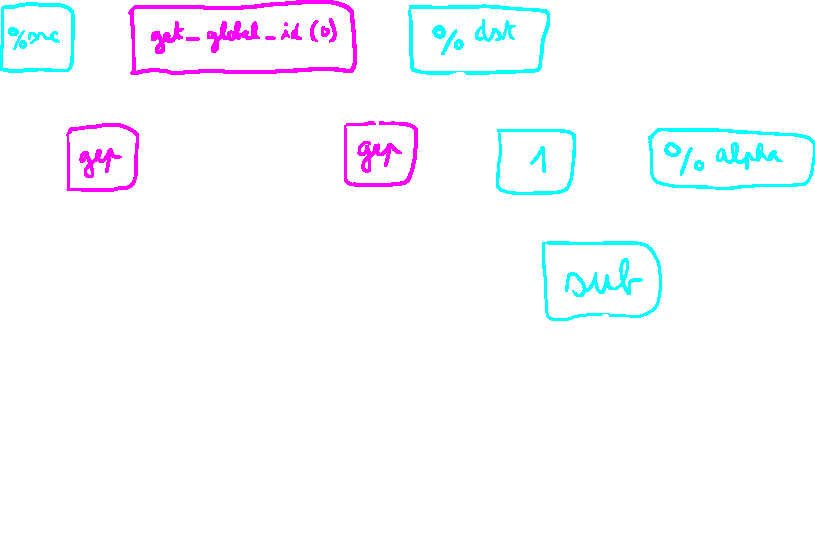
\includegraphics[scale=0.55]{images/packetization-4.pdf}}

\end{frame}

%%%%%%%%%%%%%%%%%%%%%%%%%%%%%%%%%%%%%%%%%%%%%%%%%%%%%%%%%%%%%%%%%%%%%%%%%%%%%%%%

\begin{frame}[fragile]{Packetization Example}

\begin{codebox}[commandchars=\\\[\]]
define void @__v4_add_uniform(i32* \uniform[%dst], i32* \uniform[%src], i32 \uniform[%alpha]) {
entry:
  \varying[%tid] = call i32 \varying[@get_global_id(i32 0)]
  \varying[%arrayidx] = getelementptr i32* \uniform[%src], i32 \varying[%tid]
  \varying[%0] = bitcast i32* \varying[%arrayidx] to <4 x i32>*
  \varying[%1] = load <4 x i32>* \varying[%0], align 4

  ; Broadcast (alpha - 1) to a vector
  \uniform[%sub] = sub i32 \uniform[%alpha], \uniform[1]
  \uniform[%insert] = insertelement <4 x i32> undef, i32 \uniform[%sub], i32 0
  \uniform[%broadcast_sub] = shufflevector <4 x i32> \uniform[%insert], ...

  \varying[%add] = add nsw <4 x i32> \uniform[%broadcast_sub], \varying[%1]

  \varying[%arrayidx2] = getelementptr i32* \uniform[%dst], i32 \varying[%tid]
  \varying[%2] = bitcast i32* \varying[%arrayidx2] to <4 x i32>*
  store <4 x i32> \varying[%add], <4 x i32>* \varying[%2], align 4
  ret void
}
\end{codebox}

\end{frame}
